%\documentclass[12pt]{article}
%\documentclass[12pt]{scrartcl}
\documentclass{hitec} % contained in texlive-latex-extra 
\settextfraction{0.9} % indent text
\usepackage{csquotes}
\usepackage[hidelinks]{hyperref} % doi links are short and usefull?
\hypersetup{%
    colorlinks=true,
    linkcolor=blue,
    urlcolor=magenta
}
\urlstyle{rm}
\usepackage[english]{babel}
% \usepackage[utf8]{inputenc}
% \usepackage[british,UKenglish,USenglish,american]{babel}
% \usepackage{amsmath,amsfonts,amssymb,amsthm}
\usepackage{mathtools} % loads and extends amsmath
\usepackage{amssymb}
% packages not used
%\usepackage{graphicx}
%\usepackage{amsthm}
%\usepackage{subfig}
\usepackage{bm}
\usepackage{longtable}
\usepackage{booktabs}
\usepackage{ragged2e} % maybe use \RaggedRight for tables and literature?
\usepackage[table]{xcolor} % for alternating colors
\rowcolors{2}{gray!25}{white}
\renewcommand\arraystretch{1.3}

%%% reset bibliography distances %%%
\let\oldthebibliography\thebibliography
\let\endoldthebibliography\endthebibliography
\renewenvironment{thebibliography}[1]{
  \begin{oldthebibliography}{#1}
    \RaggedRight % remove if justification is desired
    \setlength{\itemsep}{0em}
    \setlength{\parskip}{0em}
}
{
  \end{oldthebibliography}
}
%%% --- %%%

%%%%%%%%%%%%%%%%%%%%%definitions%%%%%%%%%%%%%%%%%%%%%%%%%%%%%%%%%%%%%%%
\newcommand{\eps}{\varepsilon}
\renewcommand{\d}{\mathrm{d}}
\newcommand{\T}{\mathrm{T}}
\renewcommand{\vec}[1]{{\mathbf{#1}}}
\newcommand{\dx}{\,\mathrm{d}x}
%\newcommand{\dA}{\,\mathrm{d}(x,y)}
%\newcommand{\dV}{\mathrm{d}^3{x}\,}
\newcommand{\dA}{\,\mathrm{dA}}
\newcommand{\dV}{\mathrm{dV}\,}
\newcommand{\Eins}{\mathbf{1}}
\newcommand{\ExB}{$\bm{E}\times\bm{B} \,$}
\newcommand{\GKI}{\int d^6 \bm{Z} \BSP}
\newcommand{\GKIV}{\int dv_{\|} d \mu d \theta \BSP}
\newcommand{\BSP}{B_{\|}^*}
\newcommand{\GA}[1]{\langle #1   \rangle}
\newcommand{\Abar}{\langle A_\parallel \rangle}
%Vectors
\newcommand{\bhat}{\bm{\hat{b}}}
\newcommand{\bbar}{\overline{\bm{b}}}
\newcommand{\chat}{\bm{\hat{c}}}
\newcommand{\ahat}{\bm{\hat{a}}}
\newcommand{\xhat}{\bm{\hat{x}}}
\newcommand{\yhat}{\bm{\hat{y}}}
\newcommand{\zhat}{\bm{\hat{z}}}
\newcommand{\Xbar}{\bar{\vec{X}}}
\newcommand{\phat}{\bm{\hat{\perp}}}
\newcommand{\that}{\bm{\hat{\theta}}}
\newcommand{\eI}{\bm{\hat{e}}_1}
\newcommand{\eII}{\bm{\hat{e}}_2}
\newcommand{\ud}{\mathrm{d}}
%Derivatives etc.
\newcommand{\pfrac}[2]{\frac{\partial#1}{\partial#2}}
\newcommand{\ffrac}[2]{\frac{\delta#1}{\delta#2}}
\newcommand{\fixd}[1]{\Big{\arrowvert}_{#1}}
\newcommand{\curl}[1]{\nabla \times #1}
\newcommand{\np}{\nabla_{\perp}}
\newcommand{\npc}{\nabla_{\perp} \cdot }
\newcommand{\nc}{\nabla\cdot }
\newcommand{\GAI}{\Gamma_{1}^{\dagger}}
\newcommand{\GAII}{\Gamma_{1}^{\dagger -1}}

%%%%%%%%%%%%%%%%%%%%%%%%%%%%%DOCUMENT%%%%%%%%%%%%%%%%%%%%%%%%%%%%%%%%%%%%%%%
\begin{document}

\title{BOUT, HESEL, FELTOR comparison}
\maketitle

\begin{abstract}
This document is the technical documentation of three different implementations of the same model.
\end{abstract}

\section{Model}
\subsection{Equations}
 $n$ is the electron density and $\omega$
the vorticity density. $\phi$ is the electric potential. We
use Cartesian coordinates $x$, $y$. Gyro-Bohm normalization. $\kappa$ is
the curvature, $\nu$ diffusivity.

\begin{subequations}
\begin{align}
 \nabla^2 \phi =  \omega, \quad \\
 \frac{\partial n}{\partial t}     =
    \{ n, \phi\}
  + \kappa \frac{\partial \phi}{\partial y}
  + \nu \nabla^2 n  \\
  \frac{\partial \omega}{\partial t} =
  \{ \omega, \phi\}
  - \kappa\frac{\partial n}{\partial y} +\nu\nabla^2\omega
\end{align}
\end{subequations}

For the Hasegawa - Wakatani model we the following equations

\begin{subequations}
\begin{align}
 \nabla^2 \phi =  \omega, \quad \\
 \frac{\partial n}{\partial t}     = - g \frac{\partial \phi}{\partial y} + \alpha (\tilde{\phi} - \tilde{n})
 + \{n, \phi\} + D \nabla^2 n \\
  \frac{\partial \omega}{\partial t} = \alpha ( \tilde{\phi} - \tilde{n}) + \{ \omega, \phi\}
  + \mu\nabla^2\omega
\end{align}
\end{subequations}

The variables $\tilde{\phi}$ and $\tilde{n}$ represents low frequency fluctuations. Their relation with $\phi$ and $n$ is given by

\begin{subequations}
\begin{align}
\phi = \tilde{\phi} + <\phi> \\
n = \tilde{n} + <n>
\end{align}
\end{subequations}

where $<...>$ represents the averagive in the poloidal direction. For this reason, we can write the HW model equations as 

\begin{subequations}
\begin{align}
 \nabla^2 \phi =  \omega, \quad \\
 \frac{\partial n}{\partial t}     = - g \frac{\partial \phi}{\partial y} + \alpha [(\phi - <\phi>) - (n - <n>)]
 + \{n, \phi\} + D \nabla^2 n \\
  \frac{\partial \omega}{\partial t} = \alpha [(\phi - <\phi>) - (n - <n>)]  + \{ \omega, \phi\}
  + \mu\nabla^2\omega
\end{align}
\end{subequations}

which can be approximated with $<n> \approx 0$ and $<\phi>\approx 0$.



\subsection{Domain, boundary and initial conditions}
The domain is $[0,l_x]\times[0,l_y]$.
We have periodic boundaries in $y$. In $x$ we choose homogeneous Dirichlet boundary conditions for all quantities.
Initialization of $n$ is a Gaussian
\begin{align}
    n(x,y) = A\exp\left( -\frac{(x-X)^2 + (y-Y)^2}{2\sigma^2}\right)
    \label{}
\end{align}
where $X = p_x l_x$ and $Y=p_yl_y$ with $p_x$, $p_y\in [0,1]$ are the initial centre of mass position coordinates, $A$ is the amplitude and $\sigma$ the
radius of the blob.
We initialize
\begin{align}
    \omega = \phi = 0
    \label{}
\end{align}
\subsection{Invariants}
Mass, free energy and total energy are
\begin{align*}
    M(t) := \int n \\
    F(t) := \int n^2/2 + (\nabla\phi)^2/2 \\
    H(t) := \int -\kappa nx + (\nabla\phi)^2/2
    \label{}
\end{align*}
We have
\begin{align}
  \frac{\partial}{\partial t} M &= \nu \int \nabla^2 n \\
  \frac{\partial}{\partial t} F &= \nu\int n\nabla^2 n - \phi\nabla^2\omega \\
  \frac{\partial}{\partial t} H &= - \nu \int \kappa x \nabla^2 n + \phi\nabla^2\omega
  \label{}
\end{align}

\section{Numerical methods}
\subsection{Feltor}
discontinuous Galerkin on structured grid
\begin{longtable}{ll>{\RaggedRight}p{7cm}}
\toprule
\rowcolor{gray!50}\textbf{Term} &  \textbf{Method} & \textbf{Description}  \\ \midrule
coordinate system & Cartesian 2D & equidistant discretization of $[0,l_x] \times [0,l_y]$, equal number of Gaussian nodes in x and y \\
matrix inversions & multigrid with conjugate gradient & Use previous two solutions to extrapolate initial guess \\
\ExB advection & Arakawa & s.a. \cite{Einkemmer2013} \\
curvature terms & direct & flux conserving \\
time &  Karniadakis multistep & $3rd$ order explicit, diffusion $2nd$ order implicit \\
\bottomrule
\end{longtable}

\section{Compilation and useage}

\subsection{Feltor}
There are three programs convection.cpp, convection\_hpc.cpp and convection\_mpi.cpp . Compilation with
\begin{verbatim}
make device = <omp or gpu>
\end{verbatim}
Run with
\begin{verbatim}
convection input.json
convection_hpc input.json output.nc
echo np_x np_y | mpirun -n np_x*np_y convection_mpi\
    input.json output.nc
\end{verbatim}
All programs write performance informations to std::cout.
The first opens a terminal window with live simulation results.
\begin{figure}[htpb]
\centering
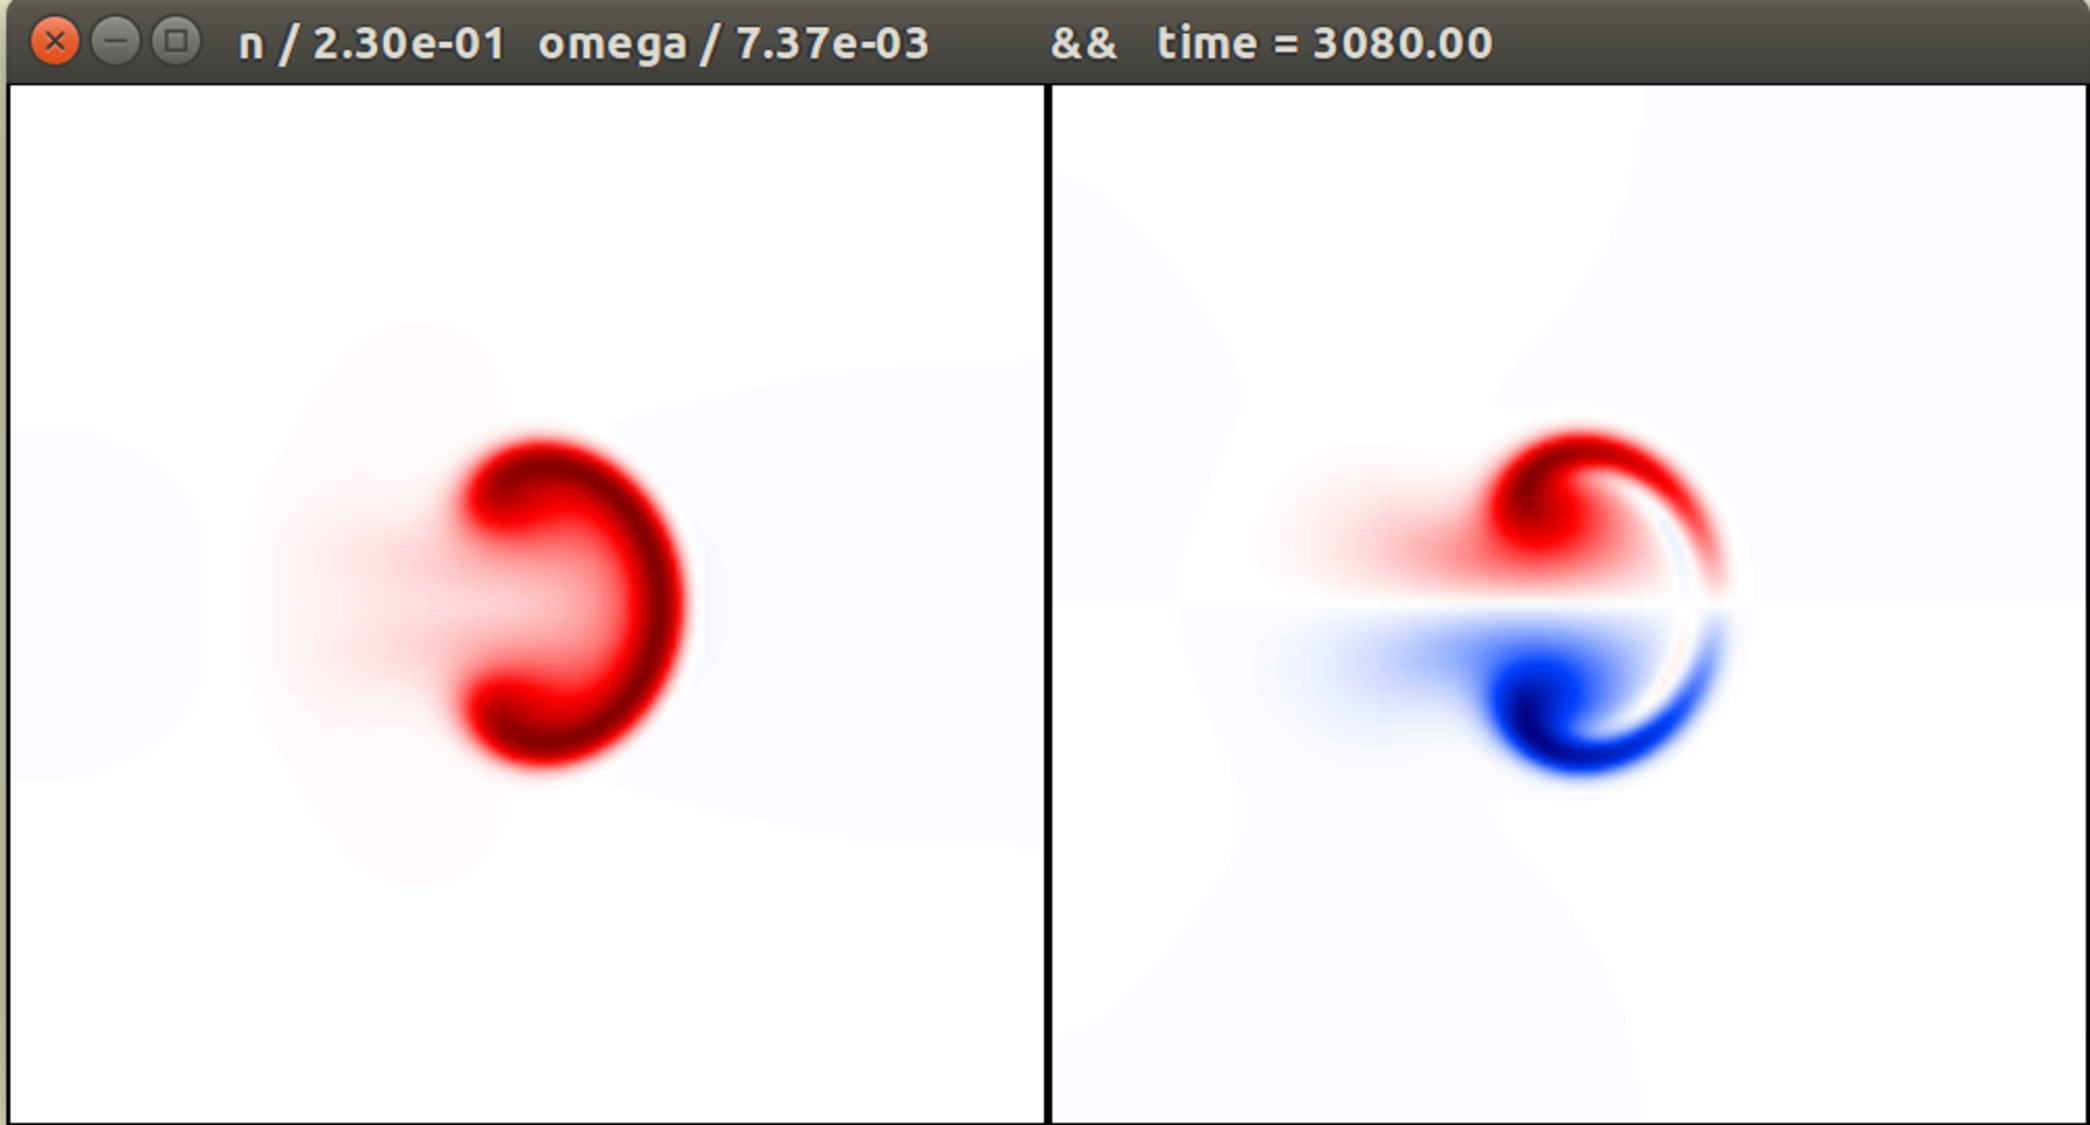
\includegraphics[trim = 0px 0px 0px 0px, clip, scale=0.4]{./blob}\label{fig:example}
\caption{
  Example blob with parameters as in the example input file.
}
\end{figure}
The other two write the results to disc.
The second is for shared memory systems. The third for distributed
memory systems, which expects the distribution of processes in the
x and y directions.

\subsubsection{Input file structure}
Input file format: json

%%This is a booktabs table
\begin{longtable}{llll>{\RaggedRight}p{7cm}}
\toprule
\rowcolor{gray!50}\textbf{Name} &  \textbf{Type} & \textbf{Example} & \textbf{Default} & \textbf{Description}  \\ \midrule
n      & integer & 3 & - &\# Gaussian nodes in x and y \\
Nx     & integer &60& - &\# grid points in x \\
Ny     & integer &60& - &\# grid points in y \\
dt     & integer &4.0& - &time step in units of $c_s/\omega_s$ \\
n\_out  & integer &3  & - &\# Gaussian nodes in x and y in output \\
Nx\_out & integer &60& - &\# grid points in x in output fields \\
Ny\_out & integer &60& - &\# grid points in y in output fields \\
itstp  & integer &10  & - &   steps between outputs \\
maxout & integer &100& - &      \# outputs excluding first \\
eps\_pol   & float &1e-6    & - &  accuracy of polarisation solver \\
eps\_time  & float &1e-10   & - & accuracy of implicit time-stepper \\
stages & integer & 3 & 3 & \# of stages in the  multigrid algorithm ( Nx and Ny have to be divisable by 2**stages) \\
curvature  & float &0.00015& - & magnetic curvature $\kappa$ \\
nu\_perp    & float &5e-3   & - & pependicular viscosity $\nu$ \\
amplitude  & float &0.5    & - & amplitude $A$ of the blob \\
sigma      & float &10     & - & blob radius $\sigma$ \\
posX       & float &0.3    & - & blob x-position in units of $l_x$, i.e. $X = p_x l_x$\\
posY       & float &0.5    & - & blob y-position in units of $l_y$, i.e. $Y = p_y l_y$ \\
lx         & float &200    & - & $l_x$  \\
ly         & float &200    & - & $l_y$  \\
bc\_x   & char & "DIR"      & - & boundary condition in x (one of PER, DIR, NEU, DIR\_NEU or NEU\_DIR) \\
bc\_y   & char & "PER"      & - & boundary condition in y (one of PER, DIR, NEU, DIR\_NEU or NEU\_DIR) \\
rows   & integer &  2 & 2 & \# of rows in window for live-plot \\
cols   & integer &  1 & 1 & \# of cols in window for live-plot \\
width  & integer & 500& 500 & width of the window in pixel in live-plot \\
height  & integer & 1000& 1000 & height of the window in pixel in live-plot \\
\bottomrule
\end{longtable}

The default value is taken if the value name is not found in the input file. If there is no default and
the value is not found,
the program exits with an error message.

\subsubsection{Structure of output file}
Output file format: netcdf-4/hdf5
%
%Name | Type | Dimensionality | Description
%---|---|---|---|
\begin{longtable}{lll>{\RaggedRight}p{7cm}}
\toprule
\rowcolor{gray!50}\textbf{Name} &  \textbf{Type} & \textbf{Dimension} & \textbf{Description}  \\ \midrule
inputfile  &             text attribute & 1 & verbose input file as a string \\
energy\_time             & Dataset & 1 & timesteps at which 1d variables are written \\
time                     & Dataset & 1 & time at which fields are written \\
x                        & Dataset & 1 & x-coordinate  \\
y                        & Dataset & 1 & y-coordinate \\
electrons                & Dataset & 3 (time, y, x) & electon density $n$ \\
ions                     & Dataset & 3 (time, y, x) & ion density $N$ or vorticity density $\omega$  \\
potential                & Dataset & 3 (time, y, x) & electric potential $\phi$  \\
vorticity                & Dataset & 3 (time, y, x) & Laplacian of potential $\nabla^2\phi$  \\
mass                     & Dataset & 1 (energy\_time) & $\int\dV n$  \\
entropy                  & Dataset & 1 (energy\_time) & $\int\dV n^2/2$  \\
kinetic                  & Dataset & 1 (energy\_time) & $\int\dV (\nabla\phi)^2//2$  \\
curvature                & Dataset & 1 (energy\_time) & $-\int\dV \kappa n x$ \\
mass\_diss               & Dataset & 1 (energy\_time) & $\nu \int\dV \nabla^2 n $  \\
entropy\_diss            & Dataset & 1 (energy\_time) & $\nu \int\dV n\nabla^2 n$  \\
kinetic\_diss            & Dataset & 1 (energy\_time) & $-\nu\int\dV\phi \nabla^2 \omega$  \\
curvature\_diss          & Dataset & 1 (energy\_time) & $-\nu\int\dV \kappa x \nabla^2 n$   \\
\bottomrule
\end{longtable}
\section{Diagnostics}
\subsection{Feltor}
%..................................................................
\begin{thebibliography}{1}
    \bibitem{Einkemmer2013}
      L. Einkemmer, M. Wiesenberger, Comput. Phys. Comm. {\bf 185} (2014) 2865-2873
\end{thebibliography}
%..................................................................


\end{document}
